\begin{frame}[t]{BERT and GPT Concepts}
  \begin{itemize}
    \item[\textcolor{red}{$\blacktriangleright$}] \textbf{BERT (Bidirectional Encoder Representations from Transformers)}
    \begin{itemize}
      \item Uses transformer encoder only.
      \item Trained with Masked Language Modeling (MLM).
      \item \textbf{Bidirectional:} Considers both left and right context.
      \item Fine-tuned for tasks like QA, classification.
      \item \textbf{Architecture:}
      \begin{itemize}
        \item Layers of encoder blocks.
        \item Positional encodings added to embeddings.
        \item Self-attention heads capture dependencies.
      \end{itemize}
    \end{itemize}
  \end{itemize}
\end{frame}

\begin{frame}{BERT -- Bidirectional Encoder Representations}
  \begin{columns}
    \begin{column}{0.58\textwidth}
      \begin{itemize}
        \item One of the biggest challenges in LM-building used to be the lack of task-specific training data.
        \vspace{1em}
        \item What if we learn an effective representation that can be applied to a variety of downstream tasks?
        \begin{itemize}
          \item Word2vec (2013)
          \item GloVe (2014)
        \end{itemize}
      \end{itemize}
    \end{column}
    \begin{column}{0.38\textwidth}
      % Placeholder for corresponding schematic/diagram
      \vspace{1em}
      \centering
      
\includegraphics[width=0.8\linewidth]{assets/Lecture-7_Large_Language_Models/pdf_page_008.png}
    \end{column}
  \end{columns}
\end{frame}

\begin{frame}{BERT -- Bidirectional Encoder Representations}
  \begin{columns}
    \begin{column}{0.56\textwidth}
      \textbf{BERT Pre-Training Corpus:}
      \begin{itemize}
        \item English Wikipedia -- 2,500 million words
        \item Book Corpus -- 800 million words
      \end{itemize}
    \end{column}
    \begin{column}{0.44\textwidth}
      % Placeholder for corresponding schematic/diagram
      \vspace{1em}
      \centering
      
\includegraphics[width=0.8\linewidth]{assets/Lecture-7_Large_Language_Models/pdf_page_008.png}
    \end{column}
  \end{columns}
\end{frame}

\begin{frame}{BERT -- Bidirectional Encoder Representations}
  \begin{columns}
    \begin{column}{0.62\textwidth}
      \textbf{BERT Pre-Training Corpus:}
      \begin{itemize}
        \item English Wikipedia -- 2,500 million words
        \item Book Corpus -- 800 million words
      \end{itemize}
      \vspace{0.7em}
      \textbf{BERT Pre-Training Tasks:}
      \begin{itemize}
        \item MLM (Masked Language Modeling)
        \item NSP (Next Sentence Prediction)
      \end{itemize}
    \end{column}
    \begin{column}{0.38\textwidth}
      % Placeholder for BERT architecture diagram
      \vspace{1em}
      \centering
      
\includegraphics[width=0.8\linewidth]{assets/Lecture-7_Large_Language_Models/pdf_page_008.png}
    \end{column}
  \end{columns}
\end{frame}

\begin{frame}{BERT -- Bidirectional Encoder Representations}
  \begin{columns}
    \begin{column}{0.62\textwidth}
      \textbf{BERT Pre-Training Corpus:}
      \begin{itemize}
        \item English Wikipedia -- 2,500 million words
        \item Book Corpus -- 800 million words
      \end{itemize}
      \vspace{0.7em}
      \textbf{BERT Pre-Training Tasks:}
      \begin{itemize}
        \item MLM (Masked Language Modeling)
        \item NSP (Next Sentence Prediction)
      \end{itemize}
      \vspace{0.7em}
      \textbf{BERT Pre-Training Results:}
      \begin{itemize}
        \item BERT-Base -- 110M Params
        \item BERT-Large -- 340M Params
      \end{itemize}
    \end{column}
    \begin{column}{0.38\textwidth}
      % Placeholder for BERT architecture diagram
      \vspace{0.5em}
      \centering
      
\includegraphics[width=0.8\linewidth]{assets/Lecture-7_Large_Language_Models/pdf_page_008.png}
    \end{column}
  \end{columns}
\end{frame}

\begin{frame}{BERT -- Bidirectional Encoder Representations}
  \centering
  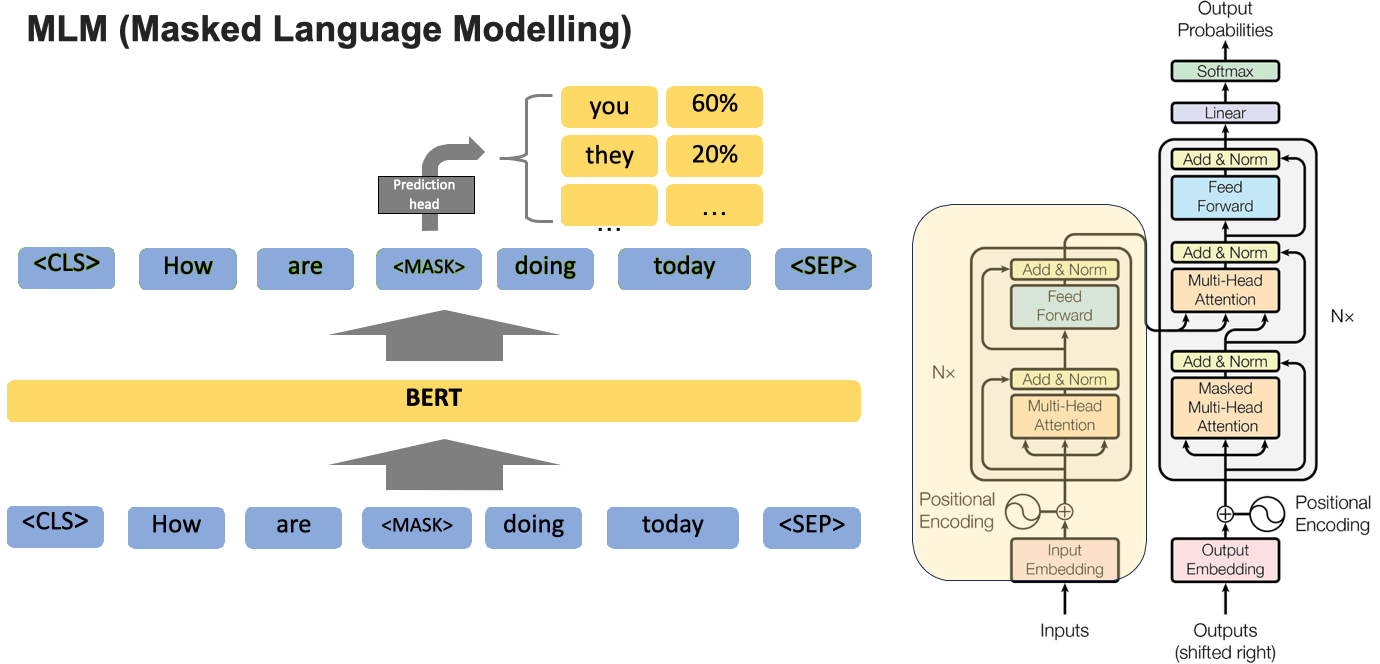
\includegraphics[width=0.60\paperwidth,height=0.60\paperheight,keepaspectratio]{assets/Lecture-7_Large_Language_Models/pdf_page_011.png}
\end{frame}

\begin{frame}{BERT -- Bidirectional Encoder Representations}
  \centering
  
\includegraphics[width=0.60\paperwidth,height=0.60\paperheight,keepaspectratio]{assets/Lecture-7_Large_Language_Models/pdf_page_012.png}
\end{frame}

\begin{frame}{BERT -- Bidirectional Encoder Representations}
  \begin{columns}
    \begin{column}{0.62\textwidth}
      \textbf{BERT Fine-Tuning:}
      \begin{itemize}
        \item Simply add a task-specific module after the last encoder layer to map it to the desired dimension.
        \item[] % extra space
        \item \textbf{\textit{Classification Tasks:}}
        \begin{itemize}
          \item Add a feed-forward layer on top of the encoder output for the [CLS] token.
        \end{itemize}
        \item[] % extra space
        \item \textbf{\textit{Question Answering Tasks:}}
        \begin{itemize}
          \item Train two extra vectors to mark the beginning and end of the answer from the paragraph.
        \end{itemize}
        \item[] 
        \item \textit{...}
      \end{itemize}
 
    \end{column}
    \begin{column}{0.38\textwidth}
      % Placeholder for BERT architecture diagram
      \vspace{0.5em}
      \centering
      
\includegraphics[width=0.8\linewidth]{assets/Lecture-7_Large_Language_Models/pdf_page_008.png}
    \end{column}
  \end{columns}
\end{frame}

% Slide 14
\begin{frame}{BERT -- Bidirectional Encoder Representations}
  \begin{columns}
    \begin{column}{0.62\textwidth}
      \textbf{BERT Evaluation:}
      \begin{itemize}
        \item \textbf{General Language Understanding Evaluation (GLUE):}
        \begin{itemize}
          \item Sentence-pair tasks --- the \emph{relationship between two sentences} (e.g.\ entailment, similarity).
          \item Single sentence classification
        \end{itemize}
        \item \textbf{Stanford Question Answering Dataset (SQuAD):}
        \begin{itemize}
          \item Tests reasoning --- answer questions whose answer is a span in a \emph{given context} paragraph.
        \end{itemize}
      \end{itemize}
    \end{column}
    \begin{column}{0.38\textwidth}
      % Placeholder for BERT architecture diagram
      \vspace{0.5em}
      \centering
      
\includegraphics[width=0.8\linewidth]{assets/Lecture-7_Large_Language_Models/pdf_page_008.png}
    \end{column}
  \end{columns}
\end{frame}

\begin{frame}{BERT -- Bidirectional Encoder Representations}
  \centering
  
\includegraphics[width=0.70\paperwidth,height=0.70\paperheight,keepaspectratio]{assets/Lecture-7_Large_Language_Models/pdf_page_015.png}
\end{frame}

\begin{frame}{BERT -- Bidirectional Encoder Representations}
  \begin{columns}
    \begin{column}{0.62\textwidth}
      \textbf{What is our takeaway from BERT?}
      \begin{itemize}
        \item \textbf{Pre-training tasks can be invented flexibly{\ldots}}
        \begin{itemize}
          \item Effective representations can be derived from a flexible regime of pre-training tasks.
        \end{itemize}
        \item \textbf{Different NLP tasks seem to be highly transferable with each other{\ldots}}
        \begin{itemize}
          \item As long as we have effective representations, that seems to form a general model which can serve as the backbone for many specialized models.
        \end{itemize}
        \item \textcolor{red}{\textbf{And scaling works!!!}}
        \begin{itemize}
          \item 340M was considered large in 2018
        \end{itemize}
      \end{itemize}
 
    \end{column}
    \begin{column}{0.38\textwidth}
      % Placeholder for BERT architecture diagram
      \vspace{0.5em}
      \centering
      
\includegraphics[width=0.8\linewidth]{assets/Lecture-7_Large_Language_Models/pdf_page_008.png}
    \end{column}
  \end{columns}
\end{frame}

\begin{frame}[t]{BERT and GPT Concepts}
  \begin{itemize}
    \item[\textcolor{red}{$\blacktriangleright$}] \textbf{GPT (Generative Pre-trained Transformer)}
    \begin{itemize}
      \item Uses transformer \textbf{decoder only}.
      \item Trained with next-token prediction.
      \item \textbf{Unidirectional:} Considers left context only.
      \item Fine-tuned for text generation, dialogue systems.
      \item \textbf{Architecture:}
      \begin{itemize}
        \item Layers of decoder blocks.
        \item Causal masking to prevent future token access.
        \item Self-attention heads capture sequential dependencies.
      \end{itemize}
    \end{itemize}
  \end{itemize}
\end{frame}

\begin{frame}{GPT -- Generative Pre-trained Transformer}
  \begin{columns}
    \begin{column}{0.62\textwidth}
      \begin{itemize}
        \item Similarly motivated as BERT, though differently designed
        \item Can we leverage large amounts of unlabeled data to pretrain an LM that understands general patterns?
      \end{itemize}
    \end{column}
    \begin{column}{0.38\textwidth}
      % Placeholder for BERT architecture diagram
      \vspace{0.5em}
      \centering
      
\includegraphics[width=0.8\linewidth]{assets/Lecture-7_Large_Language_Models/pdf_page_020.png}
    \end{column}
  \end{columns}
\end{frame}

% Slide 21
\begin{frame}{GPT -- Generative Pre-trained Transformer}
  \begin{columns}
    \begin{column}{0.62\textwidth}
      \vspace{0.5em}
      \centering
      
\includegraphics[width=0.8\linewidth]{assets/Lecture-7_Large_Language_Models/pdf_page_022.png}
    \end{column}
    \begin{column}{0.38\textwidth}
      % Placeholder for BERT architecture diagram
      \vspace{0.5em}
      \centering
      
\includegraphics[width=0.60\linewidth, height=0.60\paperheight, keepaspectratio]{assets/Lecture-7_Large_Language_Models/pdf_page_020.png}
    \end{column}
  \end{columns}
\end{frame}

\begin{frame}{GPT -- Generative Pre-trained Transformer}
  \begin{columns}
    \begin{column}{0.62\textwidth}
      \textbf{What is our takeaway from GPT?}
      \begin{itemize}
        \item \textbf{The Effectiveness of Self-Supervised Learning}
        \begin{itemize}
          \item Specifically, the model seems to be able to learn from generating the language \textit{itself}, rather than from any specific task we might cook up.
        \end{itemize}
        \item \textbf{Language Model as a Knowledge Base}
        \begin{itemize}
          \item<4-> Specifically, a generatively pre-trained model seems to have a decent zero-shot performance on a range of NLP tasks.
        \end{itemize}
        \item<5-> \textcolor{red}{\textbf{And scaling works!!!}}
      \end{itemize}
    \end{column}
    \begin{column}{0.38\textwidth}
      % Placeholder for BERT architecture diagram
      \vspace{0.5em}
      \centering
      
\includegraphics[width=0.8\linewidth]{assets/Lecture-7_Large_Language_Models/pdf_page_020.png}
    \end{column}
  \end{columns}
\end{frame}

\begin{frame}{BERT and GPT Concepts}
  \textcolor{red}{\large$\blacktriangleright$~Key Differences:}\\[1em]
  \renewcommand{\arraystretch}{1.3}
  \begin{tabular}{|l|p{3cm}|p{3cm}|}
    \hline
    \textbf{Feature}      & \textbf{BERT}                                    & \textbf{GPT}                       \\
    \hline
    Directionality        & Bidirectional                                    & Unidirectional                     \\
    \hline
    Objective             & Masked Language Modeling (MLM)                   & Causal Language Modeling (CLM)     \\
    \hline
    Output                & Contextual embeddings                            & Text generation                    \\
    \hline
    Usage                 & Fine-tuning for understanding tasks: classification, extractive QA, embeddings & Prompting for generation tasks: writing, summarization, generative QA, few-shot learning \\
    \hline
  \end{tabular}
\end{frame}
